\documentclass{article}
\usepackage[left=0.75in,top=0.6in,right=0.75in,bottom=0.6in]{geometry}
\NeedsTeXFormat{LaTeX2e}

\usepackage{hyperref}
\usepackage{xcolor}
\RequirePackage{titlesec}
\usepackage{graphicx}
\titleformat{\section}         % Customise the \section command
{\scshape\raggedright} % Can Make the \section headers large (\Large),
% small capitals (\scshape) and left aligned (\raggedright)
{}{0em}                      % Can be used to give a prefix to all sections, like 'Section ...'
{}                                                                                                                 
\titleformat{\subsection}
{\scshape\raggedright}
{}{0em}
{}
 
\newcommand{\datedsubsection}[2]{%
                \subsection[#1]{#1 \hfill #2}%
}
 
\newcommand{\name}[1]{
                \centerline{\Huge{#1}}
}
 
 
\begin{document}
\name{\textbf{Aneesh Gunda}}

\makebox[\linewidth]{\rule{\paperwidth}{2.4pt}}


%\noindent\rule[0ex]{\paperwidth}{2.4pt}


 
\begin{flushleft}
                {A-11/402 Rutu Enclave} \noindent\hspace{245}\textbf{Contact:} 9768736654%\hfill \textbf{Contact:} 9820506285\\
                \\{Anand Nagar, G.B.Road} \hfill \textbf{E-mail ID:} aneeshg96@gmail.com
                \\{Thane(w)-400615} 
                \\{Maharashtra}
                \\\hfill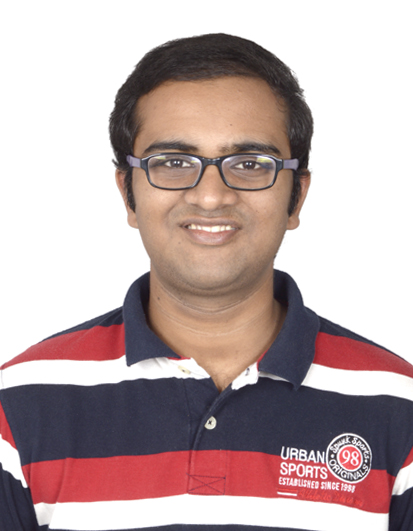
\includegraphics[width=4cm]{Aneesh}
\end{flushleft}





%===========CAREER OBJECTIVE==================================
\section{CAREER OBJECTIVE}
{\fontfamily{15}\selectfont
I wish to pursue Masters in Machine Learning and hence i would like to study deep into that domain as much as possible. 
}
%==============EDUCATION================================
\section{EDUCATION}

 
\setlength{\arrayrulewidth}{.1mm}
\setlength{\tabcolsep}{18pt}
\renewcommand{\arraystretch}{1.5}
 
%\begin{document}
\begin{tabular}{ |p{3cm}|p{3cm}|p{2cm}|p{2cm}|p{2cm}|  }
\hline

\hline
Degree or  Course & Institution & University or Board & Passing Year & Percentage\\
\hline
Undergraduate Specialization& VESIT& MU &2018& 7.62 \\
High School & Smt. Sulochanadevi Singhania School & ISC& 2014 &88\\
Secondary School & Arunodaya Public School & CBSE& 2012 & 87.8\\
\hline
\end{tabular}
%\end{document}


%======Projects=================
\section{PROJECTS}
\begin{enumerate}
               
                \item Multi Lingual Virtual Assistance Kiosk at airports for guiding people in their own preffered languages.
                \item LiFi based project to transfer audio signal via Laser.
\end{enumerate}  
%=================INTERNSHIPS=========================================
 
%\section{INTERNSHIPS}
%\begin{itemize}
%  \item One entry in the list
%  \item Another entry in the list
%\end{itemize}

%==============TECHNICAL SKILLS===================================
\section{TECHNICAL SKILLS}
\begin{itemize}
                \item Python
                \item Java
                \item Scilab
                \item C
\end{itemize}
%=============SOFT SKILLS=========================================
\section{SOFT SKILLS}
\begin{enumerate}
                \item Willingness to learn
                \item Willing to accept feedback
                \item Can work well under pressure
                
\end{enumerate}           

%===============EXTRA-CURRICULAR ACTIVITIES=========================
\section{EXTRA-CURRICULAR ACTIVITIES}
\begin{itemize}
                \item Worked for NGOs. 
                \item Participated in Cricket tournaments. 
                \item Gold medalist in karate.
                \item E-Cell representative of the Class.
\end{itemize}

%===============CO-CURRICULAR ACTIVITIES==========================
\section{CO-CURRICULAR ACTIVITIES}
\begin{enumerate}       
                \item Attended workshops on R, Matlab, Arduino.
                \item Participated in Technology Day.
                \item Won in E-Yantra Ideas Competion under Close to Market category
\end{enumerate}

%==============Personal Information=================================
\section{PERSONAL DETAILS}
{\fontfamily{15}\selectfont
 Fathers Name: Srinivas Gunda
 \\Mothers Name: Madhuri Gunda
 \\Sex: Male
 \\Date of Birth: 10th October,1996
 \\Nationality: India
 \\Marital Status: Single
}
%==============REFERENCE===========================================
\section{REFERENCES}
{\fontfamily{15}\selectfont
Dr. Mrs Gresha Bhatia
\\DHOD Computer Science Dept.
\\VESIT, Chembur, Mumbai
\\Email ID: gresha.bhatia@ves.ac.in
\\Contact Details: 09869337507
}

%============DECLARATION AND DATE==============================
\section{DECLARATION}
I HEREBY DECLARE THAT THE ABOVE RESUME IS TRUE TO THE BEST OF MY KNOWLEDGE.
\end{document}